
\subsection*{Task 0 - Joining the Slack workspace}
    
\begin{enumerate}
    \item Use the following link
    to join the Slack workspace if you are not a member yet
    \url{https://join.slack.com/t/mensacommunity/shared_invite/zt-nf09nfmb-EsChPf76BwKsUUlaRJqFqw}
    % \begin{figure}[h]
    %     \centering
    %     
\includegraphics[height=7cm]{../presentation/frame.png}
    % \end{figure}
    \item Use your email address to sign-in or use Google Sign-in
    \begin{enumerate}
    \item You might need to confirm your email address
    \item Open your email account
    \item You should have received an email from Slack (Also check your spam folder)
    \item  Click the link inside the email. 
    \end{enumerate}
    \item You should now be  in the Slack workspace
    \begin{enumerate}
        \item If you have the Slack app, you can click the popup \emph{Open in Slack}
        \item If you don't possess the Slack app, you can also use it in the browser.
    \end{enumerate}
    \item Locate the bot in the left taskbar near the bottom under Apps
    \item You can also search for the bot using the search bar on the top in the middle
\end{enumerate}

% \begin{figure}[h]
%     \centering
%     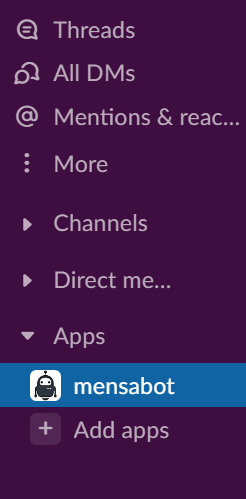
\includegraphics[height=7cm]{bot.png}
% \end{figure}


      
\subsection*{Task 1 - Getting to know the bot}
\subsubsection*{Getting the menu}
\begin{enumerate}
    \item Write a greeting message (e.g. Hello)
    \item You can type \textbf{help} to see a list of the capabilities of the bot
    \item Ask the bot to get the menu for your local mensa (canteen)
    \begin{itemize}
      \item Canteens might be closed
      \item You can also ask the bot about canteens in a particular city (e.g what is the menu for mensas in Aachen?)
      \item Try using Aachen, Mensa Academica or Aachen, Mensa Vita
    \end{itemize}
    \item The bot will look up the menu
    \item The bot might ask you if you want to set a default city. Answer with an appropriate message
\end{enumerate}
\subsubsection*{Make a review}
\begin{enumerate}
    \item Ask the bot to write a review (e.g. I want to add a review)
    \item The review process should now be starting 
    \item The bot will ask you a series of questions
    \item First specify which mensa you went to and which meal you had (e.g. I went to Aachen, Mensa Academica and had the Klassiker) 
    \begin{itemize}
      \item The spelling of the category of the dish must be in the same manner as displayed on the menu (\textbf{Klassiker, Vegetarisch} not classics or vegetarian)
    \end{itemize}
    \item Specify how many stars out of 5 you would give your meal
    \item The bot will ask you to leave a comment
    \begin{itemize}
        \item Leave an appropriate comment
        \item You can also type no if you don't want to leave a comment
      \end{itemize}
\end{enumerate}

\subsection*{Task 2 - Make a visualization}
This task involves getting insights into the success of the community. Certain success measures are predefined, which can be visualized by using the bot. Visualizations can be either a value, a chart, or a ratio.
\begin{enumerate}
    \item Ask the bot to make a visualization (e.g Make a visualization)
    \item The bot will ask for a measure. Ask the bot to list all measures
    \item Choose one of the measures 
    \begin{itemize}
        \item Copy the measure and paste it into the typing field. Then hit ENTER
    \end{itemize}
    \item The bot will respond with the appropriate visualization
    
\end{enumerate}


\subsection*{Task 3 - Update the success model}
This task involves updating the success model of the community. The success model is structured into six success \textbf{dimensions}. Each dimension contains a list of \textbf{factors}. Each factor contains a list of \textbf{measures}, which define the visualizations.
The success model is based on the requirements of the community. Those requirements were collected during the first evaluation.
\begin{enumerate}
    \item Use the bot to get the success model (e.g. Get the success model)
    % \begin{itemize}
    %     \item The bot will now list the different success dimensions
    %     \item Each dimension contains success factors
    %     \item For each factors, different measures can be listed
    % \end{itemize}
    \item Aks the bot to update the success model
    \item The bot will ask you to choose which success dimension you want to edit
    \item Choose a dimension by providing a \texttt{number}
    \item The bot will now ask you which success factor you want to edit
    \item Choose one by providing a \texttt{number} or add one by choosing a name for the factor (e.g. Customer Satisfaction)
    \item Select one of the measures. 
    \item The bot will now add the factor to the model.
    \item You can also visualize your new measure in the same way as described in Task 2
\end{enumerate}

\subsection*{Feedback}
  
\begin{enumerate}
  \item Please fill out the following survey: \url{https://limesurvey.tech4comp.dbis.rwth-aachen.de/index.php/164344?lang=en}
  \item If the link does not work, copy-paste  the one in the footnotes \footnotemark 
  \footnotetext{https://limesurvey.tech4comp.dbis.rwth-aachen.de/index.php/164344?lang=en}
\end{enumerate}